\documentclass[english,serif,mathserif,xcolor=pdftex,dvipsnames,table]{beamer}

\usepackage[T1]{fontenc}
\usepackage[utf8]{inputenc}

\usetheme[informal]{s3it}
\usepackage{s3it}

\title[Introduction to Python]{%
  A Short and Incomplete Introduction to Python
}
\subtitle{\bfseries Part 0: Introduction}
\author[S.~Haug]{%
  \textbf{Sigve Haug} \texttt{<sigve.haug@math.unibe.ch>}, \\
  Alexander Kashev \texttt{<alexander.kashev@math.unibe.ch>} \\
  Science IT Support (ScITS), University of Bern \\
  \medskip
  Based on a course by Riccardo Murri / Sergio Maffioletti
  \\
  S3IT: Services and Support for Science IT, UZH
}
\date{August 20--21, 2018}


\begin{document}

% title frame
\maketitle

\begin{frame}
  \begin{center}
    {\Huge Welcome!}
  \end{center}
\end{frame}


% \begin{frame}
%   \frametitle{What is S3IT?}

%   \begin{center}
%     {\em ``A partner for data- and \\ compute-intensive science''}

%     \+
%     \begin{description}
%     \item[Enable] researchers and projects to run simulations and data analysis.
%     \item[Develop] tools to integrate, automate and scale scientific use cases.
%     \item[Provide] access to {\em innovative} infrastructures and technologies.
%     \end{description}

%     \+
%     {\em \small{Want to know more? }\url{http://www.s3it.uzh.ch}}
%   \end{center}
% \end{frame}


\begin{frame}
  \frametitle{Prerequisites}
  Normally, a course like this assumes a basic experience with computer programming.

  \+
  Any language should do, as long as you are already familiar with
  the concepts of variables and functions.

  \+
  However, for the benefit of non-programmers, we will provide a short intro to basic concepts.

  \+
  If this applies to you, this is a helpful place to start:

  \url{https://wiki.python.org/moin/BeginnersGuide/NonProgrammers}
  
\end{frame}

\begin{frame}
  \frametitle{Why program at all?}

  \emph{``The good news about computers is that they do what you tell them to do.
  The bad news is that they do what you tell them to do.''}

  \+
  Computers are a wonderful invention, allowing to automate and accelerate
    processing of data. Like a Swiss army knife, it can be used for a great
    number of tasks.

  \+
  However, for each particular workflow computers need to be instructed
    precisely on what to do. It's the job of the \textbf{software},
    and software needs to be written.
\end{frame}

\begin{frame}
  \frametitle{Why should I program? I}

  \textbf{Automate boring, repetitive tasks.} Computers excel at mass-processing
    of data. Automating tasks can save time and reduce the number of errors.

  \+
  Some tasks are so massive in scope they cannot be solved without computers.

  \+
  \textbf{Solve my specific tasks.} Even if existing software
  can be used in solving parts of your task, perhaps no single one does it
  exactly the way you want from start to finish.
  
  \+
  If you can tie other programs together, modify them, or write your own --- you can achieve better results.
\end{frame}

\begin{frame}
  \frametitle{Why should I program? II}

  \textbf{Understanding limitations.} Non-programmers often have little idea of
  what is possible to do with computers, and how hard or easy it is.
  
  \+
  Learning programming helps you specify your requirements better, even if someone
  else will do the bulk of the work.

  \+
  \textbf{Fun.} Programming is a creative activity. If you get into it, it can be
  genuinely enjoyable to do.
  
  \+
  And if your program helps others, it's an added bonus.
\end{frame}

\begin{frame}
  \frametitle{Why Python?}

  \textbf{Relative simplicity.} Python isn't hard to install on many different systems.
  Code in Python can be simpler to express, which is great for learning.

  \+
  \textbf{High level language.} Programming with Python does not require intimate
  knowledge of how computers work, at least to start with.

  \+
  \textbf{Popularity.} Python is a very popular language. In practice,
  this means that a lot of ready recipes and tools exist for many tasks (especially scientific ones),
  and a lot of advice is available online.

\end{frame}

\begin{frame}[fragile]
  \frametitle{Python 2 \emph{vs} Python 3}

  There are currently two major versions of Python available, with
  slightly different syntax and features.

  \+
  Python 2.7 is the last release in the 2.x series.

  \+
  Python 3.x has a more polished syntax, removing inconsistencies and
  some historical baggage.

  \+
  In this course we will use \textbf{Py3 syntax}.

  \+
  {\footnotesize\em
    Watch a debate between ``Pro'' and ``Contra'' advocates:
    \url{http://www.physik.uzh.ch/~nchiapol/webm/3_1_Python3.webm}}

  \+
  {\footnotesize\em
    Explore the key differences:
    \url{http://tinyurl.com/py2-and-py3-key-differences}}
\end{frame}


% \begin{frame}
%   \frametitle{Talk outline}
%   \begin{enumerate}
%   \item Python basics
%   \item NumPy and plotting
%   %\item Pandas and how to query tabular data
%   \item Workflows with GC3Pie
%   \end{enumerate}
% \end{frame}


\begin{frame}
  \frametitle{Next steps}

  The course will be structured as a mixture of slides and hands-on
  sessions for practicing Python programming.

  \+
  So, the very first step is making sure you can access the Jupyter/IPython
  server for running the exercise notebooks.
\end{frame}


\part{How to run Python code}

\begin{frame}[fragile]
  \frametitle{The Python shell, I}
  Python is an \emph{interpreted} language.

  \+
  This means that Python code is ready to be immediately run,
  including line by line, without an initial compilation of the whole program.

  \+
  It also features an interactive
  \href{http://en.wikipedia.org/wiki/REPL}{``shell''} for evaluating
  expressions and statements immediately.

  \+
  If you have Python installed, you can use \texttt{python} to invoke
  a basic interactive shell.
\begin{semiverbatim}\tiny
\$ \textbf{python}
Python 3.6.5 |Anaconda, Inc.| (default, Apr 29 2018, 16:14:56) 
[GCC 7.2.0] on linux
Type "help", "copyright", "credits" or "license" for more information.
>{}>{}> {\color{blue}\normalfont\em \(\leftarrow\) here is where you enter commands}
\end{semiverbatim}
\end{frame}

\begin{frame}[fragile]
  \frametitle{The Python shell, II}
  The interactive mode of Python is very bare-bones.
  There are better options for interactive shells with Python.
  
  \+
  One of them is IPython, which is installed by default with Anaconda and can be installed
  as a module for other Pythons installations.

  \+
  The IPython shell is started by invoking the command
  \texttt{ipython} in a terminal window.
\begin{semiverbatim}\tiny
\$ \textbf{ipython}
Python 3.6.5 |Anaconda, Inc.| (default, Apr 29 2018, 16:14:56) 
Type 'copyright', 'credits' or 'license' for more information
IPython 6.4.0 -- An enhanced Interactive Python. Type '?' for help.

\textbf{In [1]:}{\color{blue}\normalfont\em \(\leftarrow\) here is where you enter commands}
\end{semiverbatim}
\end{frame}

\begin{frame}[fragile]
  \frametitle{Python scripts}
  Interactive mode is good for experimentation, but eventually you want
  to save your code for future reuse.

  \+
  In that case, you use a text (or code) editor to write your code in a file,
  and tell Python to run that code.

  \+
  As an obligatory first example, \textbf{hello.py:} 

\begin{semiverbatim}
print("Hello world!")
\end{semiverbatim}

  And running it:

\begin{semiverbatim}
\$ \textbf{python hello.py} 
Hello world!
\end{semiverbatim}
\end{frame}

\begin{frame}
  \frametitle{The IPython notebook, I}

  \begin{columns}[t]
    \begin{column}{0.5\textwidth}
      \begin{center}
        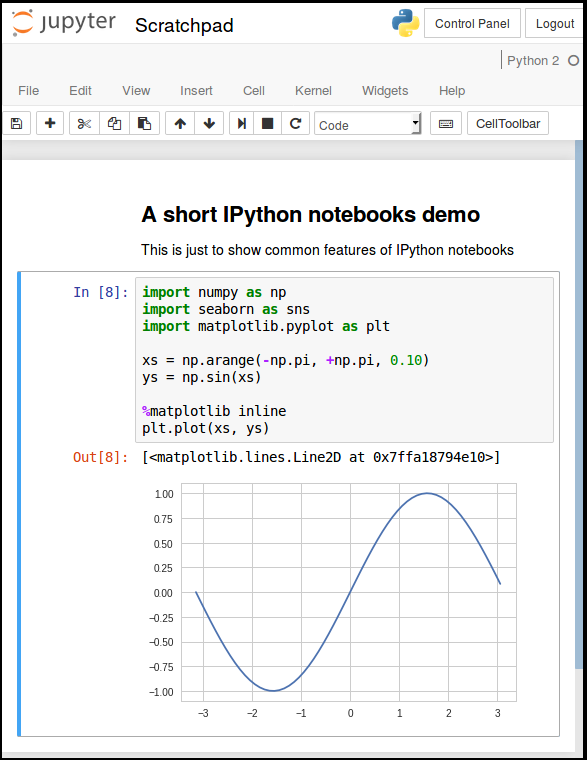
\includegraphics[width=1.00\linewidth]{fig/nb.png}
      \end{center}
    \end{column}
    \begin{column}{0.5\textwidth}
      \small

      A more appealing way of interacting with Python is through the IPython (Jupyter)
      notebooks.

      \+
      Notebooks are made of ``cells'', which come in two flavors:
      \begin{itemize}
      \item documentation cells, containing text formatted according to the
        \href{http://commonmark.org/help/}{Markdown} conventions;
      \item code cells, containing arbitrary Python code
      \end{itemize}
    \end{column}
  \end{columns}
\end{frame}


\begin{frame}
  \frametitle{The IPython notebook, II}

  Notebooks are somewhere in-between interactive shell and written and saved script.

  \+
  To run Python code in the notebook:
  \begin{itemize}
  \item Type your code in a cell besides the {\ttfamily\bfseries\color{blue}
      In~[~]:} (multiple lines are allowed)
  \item Press \textbf{Ctrl+Enter} to evaluate the cell (prompt changes to
    {\ttfamily\bfseries\color{blue} In~[*]:}) --- or press \textbf{Alt+Enter} to
    evaluate the code \emph{and} open a new code cell.
  \item When the Python kernel has done computing, the result appears \emph{under} the
    code cell marked with a {\ttfamily\bfseries\color{red} Out~[~]:} label.
  \end{itemize}

\end{frame}


\begin{frame}[fragile,fragile]
  \frametitle{The Python shell, III}
  \smaller

  Expressions can be entered at the Python shell prompt; they are evaluated and the
  result is printed:
\begin{semiverbatim}
\In 2+2
\Out 4
\end{semiverbatim}

  \+ Note that the classic Python shell uses `\texttt{>{}>{}>}' as a prompt;
  expression evaluation works exactly the same, though:
\begin{semiverbatim}
>{}>{}> 2+2
4
\end{semiverbatim}

  \+ Throughout these slides, all Python code marked with either `{\color{blue}
    In~[*]}' or `\texttt{>{}>{}>}' can also be entered and evaluated in the IPython
  notebook cells.
\end{frame}


\end{document}

%%% Local Variables:
%%% mode: latex
%%% TeX-master: t
%%% End:
